\section{ऐल्गोरिद्म}
	
	\begin{figure}[ht!]
		\hspace*{-1.8cm}
		\begin{tikzpicture}
			[node distance=1.5cm]
			
			\tikzstyle{startstop} = [rectangle, rounded corners, minimum width=3cm, minimum height=1cm,text centered, draw=black, fill=pink!30,align = center]
			
			\tikzstyle{io} = [trapezium, trapezium left angle=70, trapezium right 	angle=110, minimum width=3cm, minimum height=1cm, text centered, draw=black]
			
			\tikzstyle{process} = [rectangle, minimum width=3cm, minimum height=1cm, text 	centered, draw=black,align = center, fill = blue!20]
			
			\tikzstyle{decision} = [diamond, minimum width=3cm, minimum height=1cm, 
			align = center, draw=black, fill = green!20]
						
			\tikzstyle{arrow} = [thick,->,>=stealth]

			\node (st) [startstop] {शुरु};
			\node (pls) [process,below of=st] {led पल्स शुरू};
			\node (wt) [process, below of=pls] {0.5 सेकंड प्रतीक्षा};
			\node (findlv) [decision, below of=wt,yshift=-1cm] {$V_1$ निर्धारित स्तर\\के अन्तर्गत};
			\node (setlv) [process, left of=findlv,xshift=-3cm] {नया ड्राइव करंट सेट करें};
			\node (dc) [process, below of=findlv,yshift=-1cm] {लाल/इन्फ़रा का \\DC स्तर खोजें};
			\node (diff) [process, below of=dc] {डिफ सिग्नल उत्पन्न करें};
			\node (amp) [decision, below of=diff,yshift=-1cm] {निर्धारित स्तर\\के अन्तर्गत};
			\node (pga) [process, left of=amp,xshift=-3cm] {PGA: बढ़त चुन\\कर एम्प्लिफ़्य};
			\node (adc) [process, below of=amp,yshift=-1cm] {प्रत्येक पल्स पर\\ADC पढ़ें};
			\node (filt) [process, below of=adc] {$2^{nd}$ ऑर्डर IIR फ़िलटर};
			\node (peaks) [process, below of=filt] {शिखर - घाटी का \\पता लगाएं};
			\node (hr) [startstop,right of=peaks,xshift=+2.5cm] {HR की गणना};
			\node (ratio) [process,right of=filt,xshift=+2.5cm] {R अनुपात की गणना};
			\node (spo2) [startstop,right of=ratio,xshift=+2.5cm] {औसत $SpO_2$\& \\कि गणना};
			
			\draw [arrow] (st) -- (pls);
			\draw [arrow] (pls) -- (wt);
			\draw [arrow] (wt) -- (findlv);
			\draw [arrow] (findlv) -- node [above]{गलत} (setlv);
			\draw [arrow] (setlv) |- (pls);
			\draw [arrow] (findlv) -- node [left]{सही} (dc);
			\draw [arrow] (dc) -- (diff);
			\draw [arrow] (diff) -- (amp);
			\draw [arrow] (amp) -- node [above]{गलत} (pga);
			\draw [arrow] (amp) -- node [left]{सही} (adc);
			\draw [arrow] (pga) |- (adc);
			\draw [arrow] (adc) -- (filt);
			\draw [arrow] (filt) -- (peaks);
			\draw [arrow](peaks) -- (hr);
			\draw [arrow](filt) -- (ratio);
			\draw [arrow](ratio) -- (spo2);	
		
		
			\draw (pls) ++(3.6,0) node [align = left]{\footnotesize
			लाल$\backslash$इन्फ़्रारेड led क्रमिक\\
			\footnotesize रूप से चालु $\SI{500}{\hertz}$ पे};
			
			\draw (wt) ++(3.5,0) node [align = left]{\footnotesize
			0.5 सेकंड प्रतीक्षा PPG\\\footnotesize सिग्नल ठहराने के लिए};
			
			\draw (findlv) ++(3.7,0) node [align = left]{\footnotesize
			जाँचे PPG सिग्नल निर्धारित \\\footnotesize स्तर के अन्तर्गत नहीं तो\\
			\footnotesize नया ड्राइव करंट सेट करें};
			
			\draw (dc) ++(3.4,0) node [align = left]{\footnotesize
			लाल/इन्फ़रा DC स्तर \\\footnotesize खोजें डिफ़ सिगनल \\\footnotesize के लिये};
			
			
			\draw (diff) ++(3.6,0) node [align = left]{\footnotesize
			DAC डिफ़ सिगनल उत्पन्न \\\footnotesize करेगा DC घटाव के लिये};
			
			\draw (amp) ++(3.5,0) node [align = left]{\footnotesize
			PGA सक्षम करें यदि\\\footnotesize सिगनल स्वीकार्य स्तर के \\\footnotesize भीतर नहीं};
			
			\draw (ratio) ++(0,1) node [align = left]{\footnotesize
				R कि गणाना\\\footnotesize पडोसी समंक बिन्दुओ से};
			\draw (spo2) ++(0,1) node [align = left]{\footnotesize
				मध्यवर्ती $SpO_2$ का\\\footnotesize औसत अंतिम मूल्य के लिए};
			
		\end{tikzpicture}
		\caption{योजना प्रवाह}
	\end{figure}
	
	\subsection{IIR फ़िलटर}

		ADC से पड़े सिगनल मे शोर हो सकता है, यदि यह सिगनल सीधे शिखर - घाटी की खोज मे प्रयोग कर दिया गया, तो बहुत सारी शिखर - घाटी सटीक रूप से नहीं मिलेगा शोर के कारण। इसलिये यह ज़रुरी है कि शोर को न्यूनतम करा जा सके। 
		एक 2\textsuperscript{nd} ऑर्डर IIR फ़िलटर सिगनल को सुचारु करने के लिए पर्याप्त है। अंतर समीकरण के रूप में 2\textsuperscript{nd} ऑर्डर IIR ट्रांसफर फ़ंक्शन नीचे दिया गया है:
		
		\[
		y_i = b_1*x_i + b_2*x_{i-2} - a_2*y_{i-1} + b_3*x_{i-1} - a_3*y_{i-2}
		\]
		
		जाहा,
		
		$y_i$: मौजूदा आउटपुट
		
		$y_{i-1}$: पिछला आउटपुट
		
		$y_{i-2}$: $y_{i-1}$ का पिछला आउटपुट
		
		$x_i$: मौजूदा इनपुट
		
		$x_{i-1}$: पिछला इनपुट
		
		$x_{i-2}$: $x_{i-1}$ का पिछला इनपुट
		
		\begin{figure}[ht!]
			\centering
			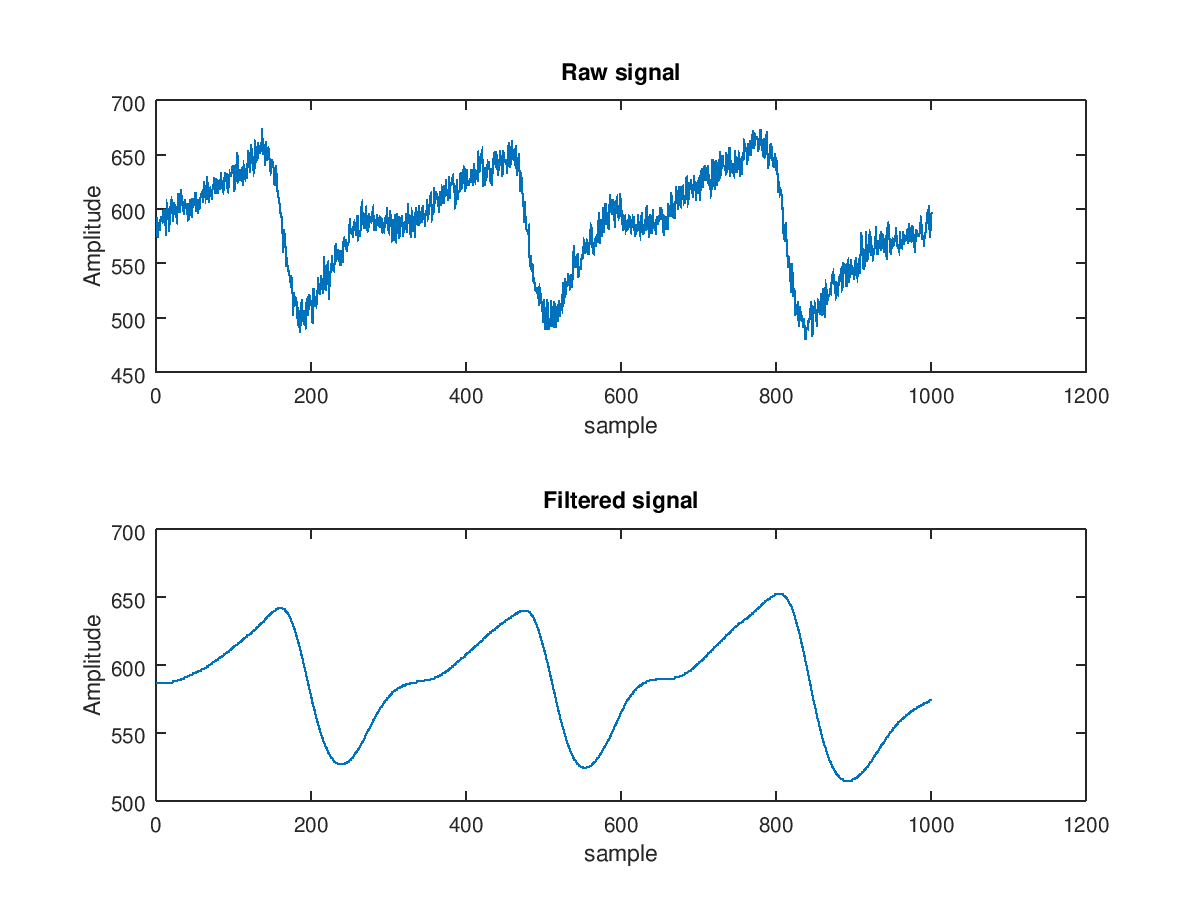
\includegraphics[width=0.8\textwidth]{../common/algo/filter.png}
			\caption{2\textsuperscript{nd} ऑर्डर बटरवर्थ IIR फ़िलटर}
			\label{fig:filter}
		\end{figure}
		
		Octave's $butter$ function\footnote{\url{https://octave.sourceforge.io/signal/function/butter.html}} का प्रयोग लो पास कॉन्फ़िगरेशन के लिए स्थानांतरण फ़ंक्शन गुणांक प्राप्त करने के लिए किया गया था।  Sampling आवृत्ति 500Hz और cut-off 3.3Hz (अधिकतम HR 200 के लिये) दिया गया था। गुणांक मान:
		
		$a_2 = -1.94137, a_3 = 0.94304$
		
		$b_1 = b_3 = 4.1762e-04$
		
		$b_2 = 8.3523e-04$	
		
		फ़िल्टर के प्रदर्शन को स्पष्ट करने के लिए, ADC से लाल सिग्नल लिया गया था, फ़िल्टर समीकरण लागू किया गया था Octave मे। जैसा कि चित्र \ref{fig:filter} में देखा गया है, फ़िल्टर शोर को दबाने में काफ़ी प्रभावी है और एक सहज आउटपुट\footnote{वास्तविक प्रोग्राम में केवल 1\textsuperscript{st} ऑर्डर फ़िल्टर लागू किया गया था क्योंकि वह अच्छा काम कर रहा था, लेकिन उपयुक्त फ़िल्टरिंग प्रदर्शन के लिए 2\textsuperscript{nd} ऑर्डर फ़िल्टर होना बहुत बेहतर है।} उत्पन्न करता है।
		
	
	\subsection{हृदय गति}
	
		हृदय गति गणना mountaineer's method for peak detection (MMPD)\cite{mmpd} ऐल्गोरिद्म से करी गयी है। 
		
		इस पद्धति में, प्रत्येक बिन्दु के लिए ढलान की गणना की जाती है और जैसे-जैसे ढलान सकारात्मक से ऋणात्मक में बदलता है, बिन्दु एक शिखर के अनुरूप होगा। इसी तरह एक ढलान का ऋणात्मक से सकारात्मक में परिवर्तन एक घाटी होगा। सकारात्मक या ऋणात्मक लगातार ढलानों के लिए एक गिनती भी ली जाती है और एक पूर्व निर्धारित मूल्य के साथ तुलना की जाती है जो ऐल्गोरिद्म की सुधार करने के लिए प्रत्येक ज्ञात शिखर के साथ अद्यतन होता है।
		
		एक टाइमर शिखर टाइमिंग को स्टोर करेगा और लगातार चोटियों के बीच समय का अंतर हृदय गति (HR) के अनुरूप होगा।
		
		\begin{figure}[ht!]
			\centering
			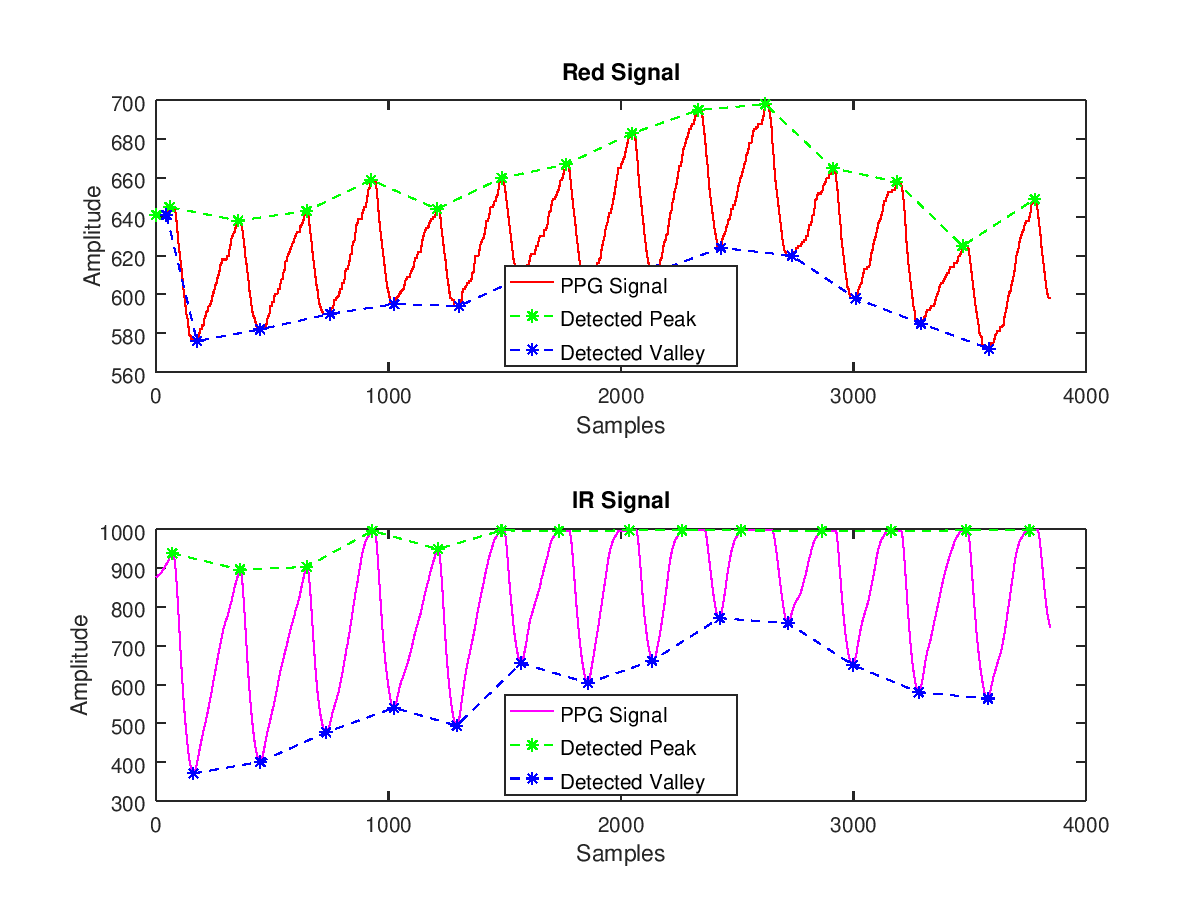
\includegraphics[width=0.7\textwidth]{../common/algo/mmpd.png}
			\caption{डेटा पर लागू ऐल्गोरिद्म}
		\end{figure}
	
	\subsection{SpO\textsubscript{2} गणना}
		
		जेसा कि पहले समीकरण \eqref{eq:calc} मे देखा गया हे:
		
		\[
			R = \sfrac{\frac{V_{p2} - V_{l2}}{DC_2}}{\frac{V_{p1} - V_{l1}}{DC_1}}
		\]	
		
		हम R कि गणना के लिए सिग्नल के वास्तविक शिखर और घाटियों का उपयोग नहीं करना चाहते हैं क्योंकि यह हृदय गति पर निर्भर है और यदि औसत निकाला जाये इस गणना से विभिन्न बिंदुओं के लिए तो अंतिम SpO\textsubscript{2}\% प्रपात करने में देरी होगी। इसलिए एक वज़न औसत विधि\cite{wuk} का उपयोग किया जाता है, जहां तात्कालिक SpO\textsubscript{2}\% की गणना पड़ोसी बिंदुओं के लिए की जाती है और एक साथ औसत करी जाती है। यह सुनिश्चित करता है कि कई तात्कालिक मूल्य प्राप्त होते हैं जिन्हें अंतिम मूल्य प्राप्त करने के लिए औसत किया जा सकता है। इस विधि मे निम्नलिखित चरणों को क्रम में किया जाता है:
		
		\begin{figure}[ht!]
			\centering
			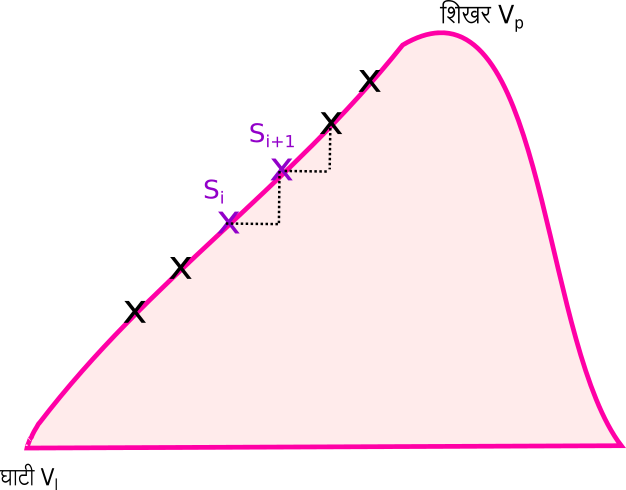
\includegraphics[width=0.5\textwidth]{images/spo2_algo.png}
			\caption{तात्कालिक SpO\textsubscript{2} के लिये चयनित बिन्दु}
		\end{figure}
	
		\begin{enumerate}
			\item लाल और इन्फ़्रारेड बिन्दुओ के क्रमागत नमूनों के बीच R प्रापत करना होगा: $S_{i+1}$ \& $S_{i}$. 
			
			\[
				R = \sfrac{\frac{S_{i_2+1} - S_{i2}}{DC_2}}{\frac{S_{i_1+1} - 		S_{i1}}{DC_1}}
			\]	
			
			इस R मान के साथ SpO\textsubscript{2} खोजें, जो एक विशिष्ट संबंध वक्र समीकरण का उपयोग करके प्राप्त किया जा सकता है जेसा कि चित्र \ref{fig:curve} मे देखा गया था:
			\[		
			SpO_2 = -25*R + 110;
			\]
			
			\item वर्तमान औसत के आधार पर इस SpO\textsubscript{2} को भार दें। यदि यह तात्कालिक SpO\textsubscript{2} औसत से कम है, तो कम भार निर्दिष्ट करें। यदि औसत के करीब है, तो अधिक भार निर्दिष्ट करें। 
			
			\item 20 बिन्दुओ के लिए भार सौंपे जाने के बाद, एक भारित औसत की गणना करें। इस भारित औसत को स्टोर करें।
			
			\item चरण 1 पर पुनरारंभ करें और ऐसे 10 पुनरावृत्तियों को निष्पादित करें।
			
			\item 10 पुनरावृत्तियों के बाद, प्रत्येक पुनरावृत्ति में परिकलित भारित औसत का औसत करे। यह अंतिम SpO\textsubscript{2} बन जाता है। इस मान को वर्तमान SpO\textsubscript{2} औसत से अपडेट करें जिसका उपयोग भार निर्दिष्ट करने के लिए किया जाता है।

		\end{enumerate}
	
		इस एल्गोरिथम का विस्तृत विवरण में मौजूद है - Pulse Oximetry: Analysis of Theory, Technology and Practise\cite{wuk}		
			
			
		अंत में, प्रत्येक 5 सेकंड में एक OLED डिस्प्ले पर SpO\textsubscript{2}\% और HR का मान प्रदर्शित किया जाता है।	